% Options for packages loaded elsewhere
\PassOptionsToPackage{unicode}{hyperref}
\PassOptionsToPackage{hyphens}{url}
%
\documentclass[
]{article}
\usepackage{amsmath,amssymb}
\usepackage{lmodern}
\usepackage{iftex}
\ifPDFTeX
  \usepackage[T1]{fontenc}
  \usepackage[utf8]{inputenc}
  \usepackage{textcomp} % provide euro and other symbols
\else % if luatex or xetex
  \usepackage{unicode-math}
  \defaultfontfeatures{Scale=MatchLowercase}
  \defaultfontfeatures[\rmfamily]{Ligatures=TeX,Scale=1}
\fi
% Use upquote if available, for straight quotes in verbatim environments
\IfFileExists{upquote.sty}{\usepackage{upquote}}{}
\IfFileExists{microtype.sty}{% use microtype if available
  \usepackage[]{microtype}
  \UseMicrotypeSet[protrusion]{basicmath} % disable protrusion for tt fonts
}{}
\makeatletter
\@ifundefined{KOMAClassName}{% if non-KOMA class
  \IfFileExists{parskip.sty}{%
    \usepackage{parskip}
  }{% else
    \setlength{\parindent}{0pt}
    \setlength{\parskip}{6pt plus 2pt minus 1pt}}
}{% if KOMA class
  \KOMAoptions{parskip=half}}
\makeatother
\usepackage{xcolor}
\usepackage[margin=1in]{geometry}
\usepackage{color}
\usepackage{fancyvrb}
\newcommand{\VerbBar}{|}
\newcommand{\VERB}{\Verb[commandchars=\\\{\}]}
\DefineVerbatimEnvironment{Highlighting}{Verbatim}{commandchars=\\\{\}}
% Add ',fontsize=\small' for more characters per line
\usepackage{framed}
\definecolor{shadecolor}{RGB}{248,248,248}
\newenvironment{Shaded}{\begin{snugshade}}{\end{snugshade}}
\newcommand{\AlertTok}[1]{\textcolor[rgb]{0.94,0.16,0.16}{#1}}
\newcommand{\AnnotationTok}[1]{\textcolor[rgb]{0.56,0.35,0.01}{\textbf{\textit{#1}}}}
\newcommand{\AttributeTok}[1]{\textcolor[rgb]{0.77,0.63,0.00}{#1}}
\newcommand{\BaseNTok}[1]{\textcolor[rgb]{0.00,0.00,0.81}{#1}}
\newcommand{\BuiltInTok}[1]{#1}
\newcommand{\CharTok}[1]{\textcolor[rgb]{0.31,0.60,0.02}{#1}}
\newcommand{\CommentTok}[1]{\textcolor[rgb]{0.56,0.35,0.01}{\textit{#1}}}
\newcommand{\CommentVarTok}[1]{\textcolor[rgb]{0.56,0.35,0.01}{\textbf{\textit{#1}}}}
\newcommand{\ConstantTok}[1]{\textcolor[rgb]{0.00,0.00,0.00}{#1}}
\newcommand{\ControlFlowTok}[1]{\textcolor[rgb]{0.13,0.29,0.53}{\textbf{#1}}}
\newcommand{\DataTypeTok}[1]{\textcolor[rgb]{0.13,0.29,0.53}{#1}}
\newcommand{\DecValTok}[1]{\textcolor[rgb]{0.00,0.00,0.81}{#1}}
\newcommand{\DocumentationTok}[1]{\textcolor[rgb]{0.56,0.35,0.01}{\textbf{\textit{#1}}}}
\newcommand{\ErrorTok}[1]{\textcolor[rgb]{0.64,0.00,0.00}{\textbf{#1}}}
\newcommand{\ExtensionTok}[1]{#1}
\newcommand{\FloatTok}[1]{\textcolor[rgb]{0.00,0.00,0.81}{#1}}
\newcommand{\FunctionTok}[1]{\textcolor[rgb]{0.00,0.00,0.00}{#1}}
\newcommand{\ImportTok}[1]{#1}
\newcommand{\InformationTok}[1]{\textcolor[rgb]{0.56,0.35,0.01}{\textbf{\textit{#1}}}}
\newcommand{\KeywordTok}[1]{\textcolor[rgb]{0.13,0.29,0.53}{\textbf{#1}}}
\newcommand{\NormalTok}[1]{#1}
\newcommand{\OperatorTok}[1]{\textcolor[rgb]{0.81,0.36,0.00}{\textbf{#1}}}
\newcommand{\OtherTok}[1]{\textcolor[rgb]{0.56,0.35,0.01}{#1}}
\newcommand{\PreprocessorTok}[1]{\textcolor[rgb]{0.56,0.35,0.01}{\textit{#1}}}
\newcommand{\RegionMarkerTok}[1]{#1}
\newcommand{\SpecialCharTok}[1]{\textcolor[rgb]{0.00,0.00,0.00}{#1}}
\newcommand{\SpecialStringTok}[1]{\textcolor[rgb]{0.31,0.60,0.02}{#1}}
\newcommand{\StringTok}[1]{\textcolor[rgb]{0.31,0.60,0.02}{#1}}
\newcommand{\VariableTok}[1]{\textcolor[rgb]{0.00,0.00,0.00}{#1}}
\newcommand{\VerbatimStringTok}[1]{\textcolor[rgb]{0.31,0.60,0.02}{#1}}
\newcommand{\WarningTok}[1]{\textcolor[rgb]{0.56,0.35,0.01}{\textbf{\textit{#1}}}}
\usepackage{graphicx}
\makeatletter
\def\maxwidth{\ifdim\Gin@nat@width>\linewidth\linewidth\else\Gin@nat@width\fi}
\def\maxheight{\ifdim\Gin@nat@height>\textheight\textheight\else\Gin@nat@height\fi}
\makeatother
% Scale images if necessary, so that they will not overflow the page
% margins by default, and it is still possible to overwrite the defaults
% using explicit options in \includegraphics[width, height, ...]{}
\setkeys{Gin}{width=\maxwidth,height=\maxheight,keepaspectratio}
% Set default figure placement to htbp
\makeatletter
\def\fps@figure{htbp}
\makeatother
\setlength{\emergencystretch}{3em} % prevent overfull lines
\providecommand{\tightlist}{%
  \setlength{\itemsep}{0pt}\setlength{\parskip}{0pt}}
\setcounter{secnumdepth}{5}
\ifLuaTeX
  \usepackage{selnolig}  % disable illegal ligatures
\fi
\IfFileExists{bookmark.sty}{\usepackage{bookmark}}{\usepackage{hyperref}}
\IfFileExists{xurl.sty}{\usepackage{xurl}}{} % add URL line breaks if available
\urlstyle{same} % disable monospaced font for URLs
\hypersetup{
  pdftitle={HUDM6122 Homework\_07},
  pdfauthor={Chenguang Pan},
  hidelinks,
  pdfcreator={LaTeX via pandoc}}

\title{HUDM6122 Homework\_07}
\author{Chenguang Pan}
\date{2023-04-12}

\begin{document}
\maketitle

\hypertarget{github-address}{%
\subsection{Github Address}\label{github-address}}

All my latest homework can be found on Github:
\url{https://github.com/cgpan/hudm6122_homeworks} . Thanks for checking
if interested.

\hypertarget{ex-7.1}{%
\subsection{Ex 7.1}\label{ex-7.1}}

\emph{In our class we mentioned the use of correlation-based distance
and Eu- clidean distance as dissimilarity measures for hierarchical
clustering. It turns out that these two measures are almost
equivalent\ldots..}

\textbf{MY SOLUTION:}

\hypertarget{solution-1-by-pure-algebra}{%
\subsubsection{Solution 1: by pure
algebra}\label{solution-1-by-pure-algebra}}

First, I prove this proportionality assumption via algebra. Then, I
validate it through data.

First, we standardized all the observations (note, not to standardize
all the variables!!). Therefore, each observation will \(X_i\) follow
\(X_i \sim N(0,1)\). That is, for any observation, we always have
\(\sigma_{X_i}=1\) and \(\mu_{X_i} =0\).

By definition, the squared the Euclidean distance can be writen as
\[d_{ij}^2 = \sum_{k=1}^{q}(x_{ik} - x_{jk})^2.\qquad\qquad \qquad...(1)\]\\
Next, we do some algebra transformations on the correlation equation,
like
\[r_{ij} = \frac{Cov(X_i,X_j)}{\sigma_{X_i}\sigma_{X_j}} =Cov(X_i,X_j)=E[(X_i-\mu_{X_i})(X_j-\mu_{X_j})]=E(X_iX_j).\qquad\qquad ...(2) \]\\
According to the definition of the expectation, we can have
\[E(X_iX_j) = \frac{\sum_{k=1}^{q}x_{ik}x_{jk}}{q}. \qquad\qquad ...(3)\]

Combine the (2) and (3), we can have
\[1-r_{ij} = 1 - \frac{1}{q}\sum_{k=1}^{q}x_{ik}x_{jk}.\qquad\qquad ...(4)\]

Back to formula (1), after expanding it, we get
\[d_{ij}^2 =\sum_{k=1}^{q}x_{ik}^2+ \sum_{k=1}^{q}x_{jk}^2 - 2\sum_{k=1}^{q}x_{ik}x_{jk}.\qquad\qquad ...(5)\]\\
Since \(X_i\) is standardized, we can easily have
\[Var(X_i) = \frac{\sum_{k=1}^{q}(x_{ik}-\mu_{X_i})^2}{q}=1. \qquad\qquad ...(6)\]\\
From the equation (6), we can prove that \(\sum_{k=1}^{q}x_{ik}^2 = q\)
and \(\sum_{k=1}^{q}x_{jk}^2 = q\). Plug these two rules into the
equation (5), we have
\[d_{ij}^2 =2q - 2\sum_{k=1}^{q}x_{ik}x_{jk}.\qquad\qquad ...(7)\]

Comparing the (4) and (7), it is not difficult to find that \(d_{ij}^2\)
is \(2q\) times that of \(1-r_{ij}.\) Note, q is the number of
variables!

In addition, if we are analyzing the sample rather than population, we
should use the unbiased estimates, which the q should be \(q-1\).
Therefore, on sample analysis, the proportion should be \(2(q-1).\)

\hypertarget{solution-2-via-data-calculation}{%
\subsubsection{Solution 2: via data
calculation}\label{solution-2-via-data-calculation}}

\begin{Shaded}
\begin{Highlighting}[]
\SpecialCharTok{\textgreater{}} \CommentTok{\# import the data}
\ErrorTok{\textgreater{}} \FunctionTok{library}\NormalTok{(}\StringTok{"HSAUR2"}\NormalTok{)}
\SpecialCharTok{\textgreater{}}\NormalTok{ df }\OtherTok{\textless{}{-}}\NormalTok{ USArrests}
\SpecialCharTok{\textgreater{}} \FunctionTok{dim}\NormalTok{(df)}
\NormalTok{[}\DecValTok{1}\NormalTok{] }\DecValTok{50}  \DecValTok{4}
\SpecialCharTok{\textgreater{}} \FunctionTok{names}\NormalTok{(df)}
\NormalTok{[}\DecValTok{1}\NormalTok{] }\StringTok{"Murder"}   \StringTok{"Assault"}  \StringTok{"UrbanPop"} \StringTok{"Rape"}    
\SpecialCharTok{\textgreater{}} 
\ErrorTok{\textgreater{}} \CommentTok{\# standardize the observations}
\ErrorTok{\textgreater{}}\NormalTok{ df\_matrix }\OtherTok{\textless{}{-}} \FunctionTok{as.matrix}\NormalTok{(df)}
\SpecialCharTok{\textgreater{}}\NormalTok{ df\_mat\_obs\_std }\OtherTok{\textless{}{-}} \FunctionTok{t}\NormalTok{(}\FunctionTok{scale}\NormalTok{(}\FunctionTok{t}\NormalTok{(df\_matrix)))}
\SpecialCharTok{\textgreater{}} 
\ErrorTok{\textgreater{}} \CommentTok{\# randomly choose two rows}
\ErrorTok{\textgreater{}}\NormalTok{ rand\_idx }\OtherTok{\textless{}{-}} \FunctionTok{sample}\NormalTok{(}\DecValTok{1}\SpecialCharTok{:}\FunctionTok{nrow}\NormalTok{(df\_mat\_obs\_std),}\DecValTok{2}\NormalTok{)}
\SpecialCharTok{\textgreater{}} \CommentTok{\# calculate the Euclidean distance}
\ErrorTok{\textgreater{}}\NormalTok{ d\_ }\OtherTok{\textless{}{-}} \FunctionTok{dist}\NormalTok{(df\_mat\_obs\_std[rand\_idx,])}
\SpecialCharTok{\textgreater{}}\NormalTok{ d\_sqr }\OtherTok{\textless{}{-}} \FunctionTok{as.numeric}\NormalTok{(d\_}\SpecialCharTok{\^{}}\DecValTok{2}\NormalTok{)}
\SpecialCharTok{\textgreater{}} \CommentTok{\# calcualte the correlation }
\ErrorTok{\textgreater{}}\NormalTok{ r\_ }\OtherTok{\textless{}{-}} \FunctionTok{cor}\NormalTok{(df\_mat\_obs\_std[rand\_idx[}\DecValTok{1}\NormalTok{],],}
\SpecialCharTok{+}\NormalTok{           df\_mat\_obs\_std[rand\_idx[}\DecValTok{2}\NormalTok{],])}
\SpecialCharTok{\textgreater{}} \CommentTok{\# q here is 4. }
\ErrorTok{\textgreater{}}\NormalTok{ d\_sqr}\SpecialCharTok{/}\NormalTok{(}\DecValTok{1}\SpecialCharTok{{-}}\NormalTok{r\_)}
\NormalTok{[}\DecValTok{1}\NormalTok{] }\DecValTok{6}
\end{Highlighting}
\end{Shaded}

The number of variables here is 4, since it is the sample analysis, the
proportion should be \(2(q-1)= 6\), which is exactly the same to our
algebra analysis!

\hypertarget{ex-7.2}{%
\subsection{Ex 7.2}\label{ex-7.2}}

\emph{Section 3.3 on page 65 gives a formula for calculating the
proportion of the total variation (PTV) explained by the principal
components\ldots..}

\textbf{MY SOLUTION:}

\begin{Shaded}
\begin{Highlighting}[]
\SpecialCharTok{\textgreater{}} \CommentTok{\# run pca first}
\ErrorTok{\textgreater{}}\NormalTok{ df\_pca }\OtherTok{\textless{}{-}} \FunctionTok{prcomp}\NormalTok{(df, }\AttributeTok{scale=}\ConstantTok{TRUE}\NormalTok{)}
\SpecialCharTok{\textgreater{}} \FunctionTok{summary}\NormalTok{(df\_pca)}
\NormalTok{Importance of components}\SpecialCharTok{:}
\NormalTok{                          PC1    PC2     PC3     PC4}
\NormalTok{Standard deviation     }\FloatTok{1.5749} \FloatTok{0.9949} \FloatTok{0.59713} \FloatTok{0.41645}
\NormalTok{Proportion of Variance }\FloatTok{0.6201} \FloatTok{0.2474} \FloatTok{0.08914} \FloatTok{0.04336}
\NormalTok{Cumulative Proportion  }\FloatTok{0.6201} \FloatTok{0.8675} \FloatTok{0.95664} \FloatTok{1.00000}
\end{Highlighting}
\end{Shaded}

\begin{Shaded}
\begin{Highlighting}[]
\SpecialCharTok{\textgreater{}} \CommentTok{\# extract the sd of each component}
\ErrorTok{\textgreater{}}\NormalTok{ var\_sets }\OtherTok{\textless{}{-}}\NormalTok{ df\_pca}\SpecialCharTok{$}\NormalTok{sdev}\SpecialCharTok{\^{}}\DecValTok{2}
\SpecialCharTok{\textgreater{}} \CommentTok{\# calculate the sum of the total variance}
\ErrorTok{\textgreater{}}\NormalTok{ total\_var }\OtherTok{\textless{}{-}} \FunctionTok{sum}\NormalTok{(var\_sets)}
\SpecialCharTok{\textgreater{}} \CommentTok{\# calculate the PTV for each component}
\ErrorTok{\textgreater{}}\NormalTok{ (ptv\_1 }\OtherTok{\textless{}{-}}\NormalTok{ var\_sets[}\DecValTok{1}\NormalTok{]}\SpecialCharTok{/}\NormalTok{total\_var)}
\NormalTok{[}\DecValTok{1}\NormalTok{] }\FloatTok{0.6200604}
\SpecialCharTok{\textgreater{}}\NormalTok{ (ptv\_2 }\OtherTok{\textless{}{-}}\NormalTok{ var\_sets[}\DecValTok{2}\NormalTok{]}\SpecialCharTok{/}\NormalTok{total\_var)}
\NormalTok{[}\DecValTok{1}\NormalTok{] }\FloatTok{0.2474413}
\SpecialCharTok{\textgreater{}}\NormalTok{ (ptv\_3 }\OtherTok{\textless{}{-}}\NormalTok{ var\_sets[}\DecValTok{3}\NormalTok{]}\SpecialCharTok{/}\NormalTok{total\_var)}
\NormalTok{[}\DecValTok{1}\NormalTok{] }\FloatTok{0.0891408}
\SpecialCharTok{\textgreater{}}\NormalTok{ (ptv\_4 }\OtherTok{\textless{}{-}}\NormalTok{ var\_sets[}\DecValTok{4}\NormalTok{]}\SpecialCharTok{/}\NormalTok{total\_var)}
\NormalTok{[}\DecValTok{1}\NormalTok{] }\FloatTok{0.04335752}
\end{Highlighting}
\end{Shaded}

The result is exactly the same to the PTV given by the pca results.

\hypertarget{ex-7.3}{%
\subsection{Ex 7.3}\label{ex-7.3}}

\emph{We aim at performing hierarchical clustering on the states.}

\hypertarget{a}{%
\subsubsection{7.3.a}\label{a}}

\emph{Using hierarchical clustering with complete linkage and Euclidean
distance, cluster the states.}

\textbf{MY SOLUTION:}

\begin{Shaded}
\begin{Highlighting}[]
\SpecialCharTok{\textgreater{}} \CommentTok{\# get the distance matrix}
\ErrorTok{\textgreater{}}\NormalTok{ dm }\OtherTok{\textless{}{-}} \FunctionTok{dist}\NormalTok{(df)}
\SpecialCharTok{\textgreater{}} \CommentTok{\# run the hierarchical clustering}
\ErrorTok{\textgreater{}}\NormalTok{ cc }\OtherTok{\textless{}{-}} \FunctionTok{hclust}\NormalTok{(dm,}\AttributeTok{method =} \StringTok{"complete"}\NormalTok{)}
\end{Highlighting}
\end{Shaded}

\hypertarget{b}{%
\subsubsection{7.3.b}\label{b}}

\emph{Cut the dendrogram at a height that results in three distinct
clusters. Which states belong to which clusters?}

\textbf{MY SOLUTION:}

\begin{Shaded}
\begin{Highlighting}[]
\SpecialCharTok{\textgreater{}} \CommentTok{\# plot the deprogram}
\ErrorTok{\textgreater{}} \FunctionTok{plot}\NormalTok{(cc)}
\SpecialCharTok{\textgreater{}} \FunctionTok{abline}\NormalTok{(}\AttributeTok{h=}\DecValTok{130}\NormalTok{, }\AttributeTok{col=}\StringTok{"blue"}\NormalTok{)}
\end{Highlighting}
\end{Shaded}

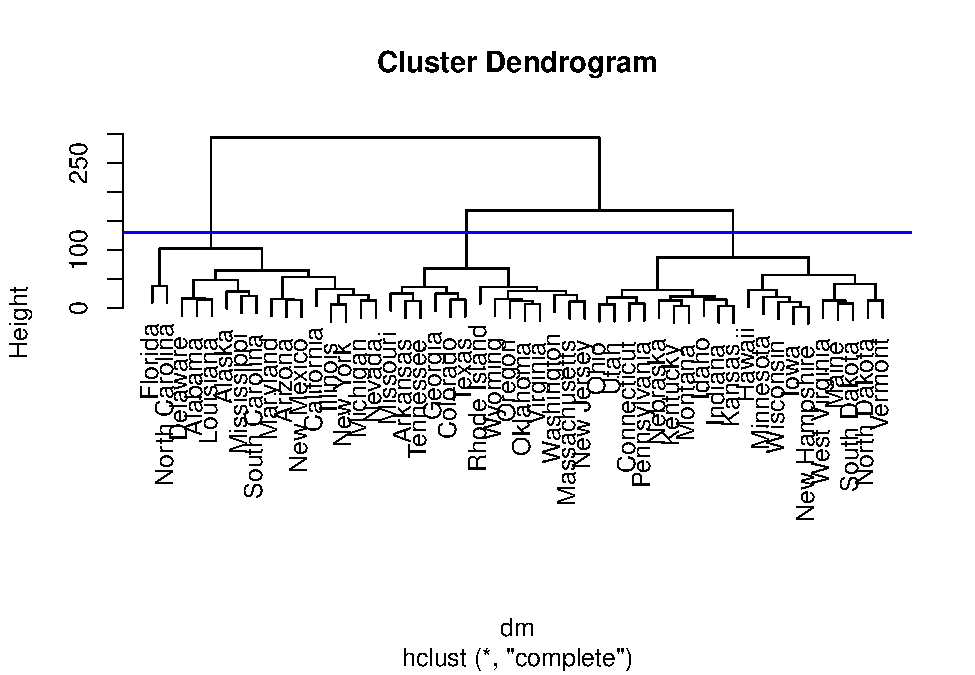
\includegraphics{HUDM6122-Homework_07-Chenguang-Pan_files/figure-latex/unnamed-chunk-5-1.pdf}

\hypertarget{c}{%
\subsubsection{7.3.c}\label{c}}

\emph{Hierarchically cluster the states using complete linkage and
Euclidean distance, after scaling the variables to have standard
deviation one.}

\textbf{MY SOLUTION:}

\begin{Shaded}
\begin{Highlighting}[]
\SpecialCharTok{\textgreater{}} \CommentTok{\# I choose to standardize all columns}
\ErrorTok{\textgreater{}}\NormalTok{ X }\OtherTok{\textless{}{-}} \FunctionTok{scale}\NormalTok{(df, }\AttributeTok{center =}\NormalTok{ T, }\AttributeTok{scale =}\NormalTok{ T)}
\SpecialCharTok{\textgreater{}}\NormalTok{ dmX }\OtherTok{\textless{}{-}} \FunctionTok{dist}\NormalTok{(X)}
\SpecialCharTok{\textgreater{}}\NormalTok{ ccX }\OtherTok{\textless{}{-}} \FunctionTok{hclust}\NormalTok{(dmX,}\AttributeTok{method =} \StringTok{"complete"}\NormalTok{)}
\SpecialCharTok{\textgreater{}} \FunctionTok{plot}\NormalTok{(ccX)}
\SpecialCharTok{\textgreater{}} \FunctionTok{abline}\NormalTok{(}\AttributeTok{h=}\FloatTok{3.9}\NormalTok{, }\AttributeTok{col=}\StringTok{"blue"}\NormalTok{)}
\end{Highlighting}
\end{Shaded}

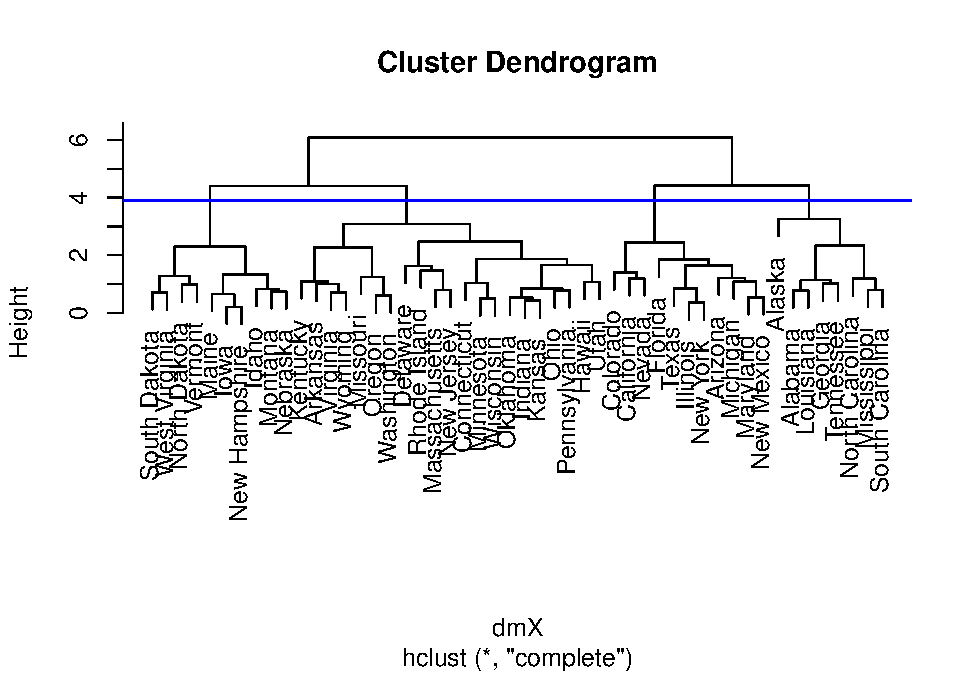
\includegraphics{HUDM6122-Homework_07-Chenguang-Pan_files/figure-latex/unnamed-chunk-6-1.pdf}

\hypertarget{d}{%
\subsubsection{7.3.d}\label{d}}

\emph{What effect does scaling the variables have on the hierarchical
clus- tering obtained?}

\textbf{MY SOLUTION:}

Comparing the plots from (b) and (c), one can see that the results are
different after running with same method. After checking on the raw
data, we can see that the variables are at different scales. One should
notice that the Euclidean distance is sensitive to the scaling of
variable. That is, a large difference in one dimension can have a
disproportionate effect on the overall distance, even if the differences
in the other dimensions are relatively small. To avoid this limitation,
I suggest that we should standardize the raw data if they are on
different scales.

\end{document}
